\documentclass[a4paper]{article}
\usepackage[a4paper, total={7in, 8in}]{geometry}
%\pdfoptionpdfminorversion=5

\usepackage{graphicx}
\usepackage{amsmath}

\begin{document}

\title{Exponential-function}
\author{Anne Rasmussen}
\maketitle


\section{Introduction}

The exponential function is a mathematical function denoted by
$f(x)=\exp(x)$ or $e^x$. The formal definition of the exponential function is: 

\begin{equation}
\exp x := \sum_{k = 0}^{\infty} \frac{x^k}{k!} = 1 + x + \frac{x^2}{2} + \frac{x^3}{6} + \frac{x^4}{24} + \cdots
\end{equation}

This is an infinite sum. Here we approximate the exponential function by: 

\begin{equation} \label{eq:approx_exp}
\exp x \approx 1+x*\left(1+\frac{x}{2}*\left(1+\frac{x}{3}*\left(1+\frac{x}{4}*\left(1+\frac{x}{5}*\left(1+\frac{x}{6}*\left(1+\frac{x}{7}*\left(1+\frac{x}{8}*\left(1+\frac{x}{9}*\left(1+\frac{x}{10}\right)\right)\right)\right)\right)\right)\right)\right)\right)
\end{equation}

\begin{figure}[!h]
\centering
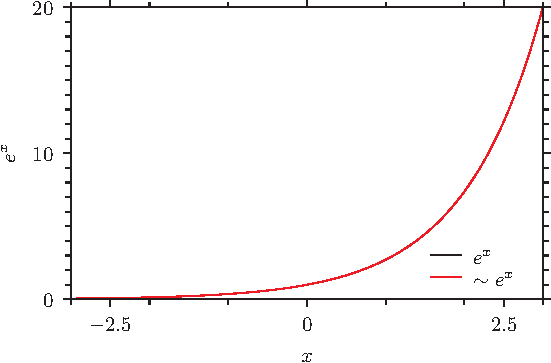
\includegraphics{exp.pdf}
\caption{The exponential function. The black line is the exponential funciton using the System.Math and the red line is the approximate exponential function found from equation \eqref{eq:approx_exp}}
\end{figure}


\end{document}

